\documentclass[twoside]{book}

% Packages required by doxygen
\usepackage{fixltx2e}
\usepackage{calc}
\usepackage{doxygen}
\usepackage[export]{adjustbox} % also loads graphicx
\usepackage{graphicx}
\usepackage[utf8]{inputenc}
\usepackage{makeidx}
\usepackage{multicol}
\usepackage{multirow}
\PassOptionsToPackage{warn}{textcomp}
\usepackage{textcomp}
\usepackage[nointegrals]{wasysym}
\usepackage[table]{xcolor}

% Font selection
\usepackage[T1]{fontenc}
\usepackage[scaled=.90]{helvet}
\usepackage{courier}
\usepackage{amssymb}
\usepackage{sectsty}
\renewcommand{\familydefault}{\sfdefault}
\allsectionsfont{%
  \fontseries{bc}\selectfont%
  \color{darkgray}%
}
\renewcommand{\DoxyLabelFont}{%
  \fontseries{bc}\selectfont%
  \color{darkgray}%
}
\newcommand{\+}{\discretionary{\mbox{\scriptsize$\hookleftarrow$}}{}{}}

% Page & text layout
\usepackage{geometry}
\geometry{%
  a4paper,%
  top=2.5cm,%
  bottom=2.5cm,%
  left=2.5cm,%
  right=2.5cm%
}
\tolerance=750
\hfuzz=15pt
\hbadness=750
\setlength{\emergencystretch}{15pt}
\setlength{\parindent}{0cm}
\setlength{\parskip}{3ex plus 2ex minus 2ex}
\makeatletter
\renewcommand{\paragraph}{%
  \@startsection{paragraph}{4}{0ex}{-1.0ex}{1.0ex}{%
    \normalfont\normalsize\bfseries\SS@parafont%
  }%
}
\renewcommand{\subparagraph}{%
  \@startsection{subparagraph}{5}{0ex}{-1.0ex}{1.0ex}{%
    \normalfont\normalsize\bfseries\SS@subparafont%
  }%
}
\makeatother

% Headers & footers
\usepackage{fancyhdr}
\pagestyle{fancyplain}
\fancyhead[LE]{\fancyplain{}{\bfseries\thepage}}
\fancyhead[CE]{\fancyplain{}{}}
\fancyhead[RE]{\fancyplain{}{\bfseries\leftmark}}
\fancyhead[LO]{\fancyplain{}{\bfseries\rightmark}}
\fancyhead[CO]{\fancyplain{}{}}
\fancyhead[RO]{\fancyplain{}{\bfseries\thepage}}
\fancyfoot[LE]{\fancyplain{}{}}
\fancyfoot[CE]{\fancyplain{}{}}
\fancyfoot[RE]{\fancyplain{}{\bfseries\scriptsize Generated by Doxygen }}
\fancyfoot[LO]{\fancyplain{}{\bfseries\scriptsize Generated by Doxygen }}
\fancyfoot[CO]{\fancyplain{}{}}
\fancyfoot[RO]{\fancyplain{}{}}
\renewcommand{\footrulewidth}{0.4pt}
\renewcommand{\chaptermark}[1]{%
  \markboth{#1}{}%
}
\renewcommand{\sectionmark}[1]{%
  \markright{\thesection\ #1}%
}

% Indices & bibliography
\usepackage{natbib}
\usepackage[titles]{tocloft}
\setcounter{tocdepth}{3}
\setcounter{secnumdepth}{5}
\makeindex

% Hyperlinks (required, but should be loaded last)
\usepackage{ifpdf}
\ifpdf
  \usepackage[pdftex,pagebackref=true]{hyperref}
\else
  \usepackage[ps2pdf,pagebackref=true]{hyperref}
\fi
\hypersetup{%
  colorlinks=true,%
  linkcolor=blue,%
  citecolor=blue,%
  unicode%
}

% Custom commands
\newcommand{\clearemptydoublepage}{%
  \newpage{\pagestyle{empty}\cleardoublepage}%
}

\usepackage{caption}
\captionsetup{labelsep=space,justification=centering,font={bf},singlelinecheck=off,skip=4pt,position=top}

%===== C O N T E N T S =====

\begin{document}

% Titlepage & ToC
\hypersetup{pageanchor=false,
             bookmarksnumbered=true,
             pdfencoding=unicode
            }
\pagenumbering{roman}
\begin{titlepage}
\vspace*{7cm}
\begin{center}%
{\Large 42sh }\\
\vspace*{1cm}
{\large Generated by Doxygen 1.8.11}\\
\end{center}
\end{titlepage}
\clearemptydoublepage
\tableofcontents
\clearemptydoublepage
\pagenumbering{arabic}
\hypersetup{pageanchor=true}

%--- Begin generated contents ---
\chapter{File Index}
\section{File List}
Here is a list of all documented files with brief descriptions\+:\begin{DoxyCompactList}
\item\contentsline{section}{src/\hyperlink{main_8c}{main.\+c} \\*Program for the main }{\pageref{main_8c}}{}
\end{DoxyCompactList}

\chapter{File Documentation}
\hypertarget{main_8c}{}\section{src/main.c File Reference}
\label{main_8c}\index{src/main.\+c@{src/main.\+c}}


Program for the main.  


{\ttfamily \#include $<$stdio.\+h$>$}\\*
{\ttfamily \#include $<$fcntl.\+h$>$}\\*
{\ttfamily \#include $<$unistd.\+h$>$}\\*
{\ttfamily \#include $<$string.\+h$>$}\\*
{\ttfamily \#include $<$sys/mman.\+h$>$}\\*
{\ttfamily \#include $<$err.\+h$>$}\\*
{\ttfamily \#include $<$stdlib.\+h$>$}\\*
{\ttfamily \#include $<$sys/stat.\+h$>$}\\*
{\ttfamily \#include $<$getopt.\+h$>$}\\*
{\ttfamily \#include \char`\"{}include/shell.\+h\char`\"{}}\\*
{\ttfamily \#include \char`\"{}lexer/include/lexer\+\_\+struct.\+h\char`\"{}}\\*
{\ttfamily \#include \char`\"{}lexer/include/my\+\_\+tree.\+h\char`\"{}}\\*
{\ttfamily \#include \char`\"{}lexer/include/rule.\+h\char`\"{}}\\*
{\ttfamily \#include \char`\"{}print\+\_\+ast/include/print\+\_\+ast.\+h\char`\"{}}\\*
Include dependency graph for main.\+c\+:\nopagebreak
\begin{figure}[H]
\begin{center}
\leavevmode
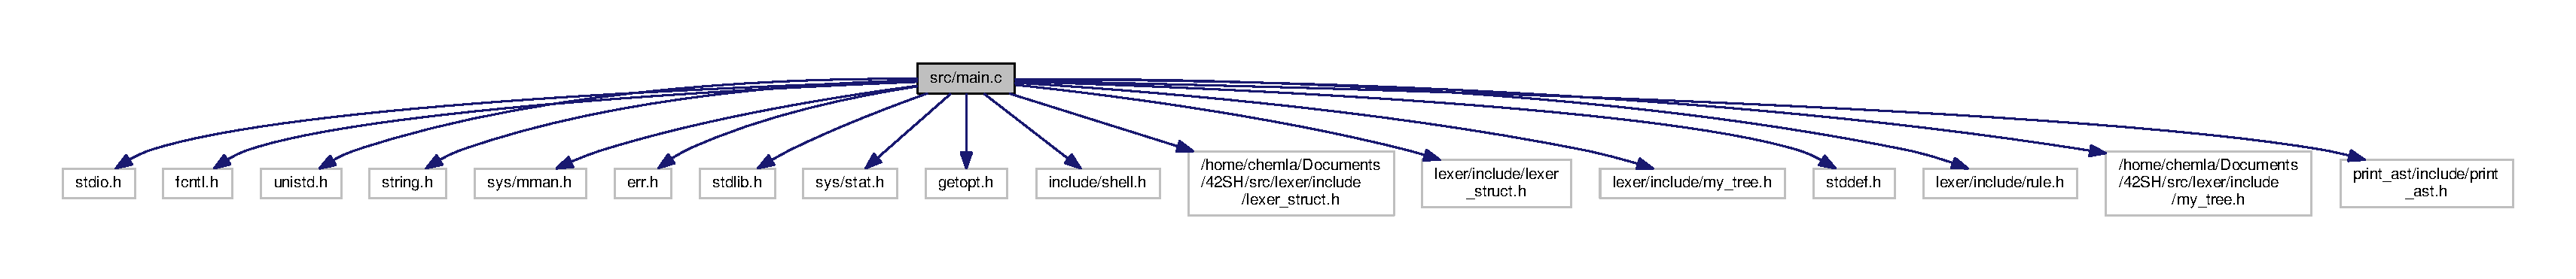
\includegraphics[width=350pt]{main_8c__incl}
\end{center}
\end{figure}
\subsection*{Functions}
\begin{DoxyCompactItemize}
\item 
void {\bfseries add\+\_\+token} (struct Token $\ast$$\ast$token, char $\ast$str)\hypertarget{main_8c_afb84c62a61e5423683cd14dcd09869a1}{}\label{main_8c_afb84c62a61e5423683cd14dcd09869a1}

\item 
struct Token $\ast$ {\bfseries parse\+\_\+path} (struct Token $\ast$token, char $\ast$$\ast$argv, long argc, struct PS $\ast$ps)\hypertarget{main_8c_ab4dceacddf2678165fe46683f4346035}{}\label{main_8c_ab4dceacddf2678165fe46683f4346035}

\item 
void \hyperlink{main_8c_a896ebd9330a9cd0214cb899a28bcae76}{print\+\_\+t} (struct Token $\ast$t)
\begin{DoxyCompactList}\small\item\em Printing A\+ST function. \end{DoxyCompactList}\item 
struct Token $\ast$ {\bfseries lexer} (struct Token $\ast$t)\hypertarget{main_8c_a2ff68d8e74fe500262ae39dfe782d66e}{}\label{main_8c_a2ff68d8e74fe500262ae39dfe782d66e}

\item 
void {\bfseries Destroy\+Token} (struct Token $\ast$t)\hypertarget{main_8c_a20e488f2f61f0493ae9fa3da87def064}{}\label{main_8c_a20e488f2f61f0493ae9fa3da87def064}

\item 
struct PS $\ast$ {\bfseries init\+\_\+ps} (void)\hypertarget{main_8c_accf36cd1c7e073ad43ea9074ff2ac8b3}{}\label{main_8c_accf36cd1c7e073ad43ea9074ff2ac8b3}

\item 
struct Token $\ast$ {\bfseries carving} (long argc, char $\ast$$\ast$argv)\hypertarget{main_8c_a07fcb75e60a631eaf3cd1c6612620a06}{}\label{main_8c_a07fcb75e60a631eaf3cd1c6612620a06}

\item 
int {\bfseries main} (int argc, char $\ast$argv\mbox{[}$\,$\mbox{]})\hypertarget{main_8c_a0ddf1224851353fc92bfbff6f499fa97}{}\label{main_8c_a0ddf1224851353fc92bfbff6f499fa97}

\end{DoxyCompactItemize}


\subsection{Detailed Description}
Program for the main. 


\begin{DoxyItemize}
\item \begin{DoxyVersion}{Version}
0.\+5 
\end{DoxyVersion}
\begin{DoxyDate}{Date}
30 novembre 2018
\end{DoxyDate}
File with the main 
\end{DoxyItemize}

\subsection{Function Documentation}
\index{main.\+c@{main.\+c}!print\+\_\+t@{print\+\_\+t}}
\index{print\+\_\+t@{print\+\_\+t}!main.\+c@{main.\+c}}
\subsubsection[{\texorpdfstring{print\+\_\+t(struct Token $\ast$t)}{print_t(struct Token *t)}}]{\setlength{\rightskip}{0pt plus 5cm}void print\+\_\+t (
\begin{DoxyParamCaption}
\item[{struct Token $\ast$}]{t}
\end{DoxyParamCaption}
)}\hypertarget{main_8c_a896ebd9330a9cd0214cb899a28bcae76}{}\label{main_8c_a896ebd9330a9cd0214cb899a28bcae76}


Printing A\+ST function. 


\begin{DoxyParams}{Parameters}
{\em t} & Adress of the pointer structure to be print. \\
\hline
\end{DoxyParams}
\begin{DoxyReturn}{Returns}
No return. 
\end{DoxyReturn}

%--- End generated contents ---

% Index
\backmatter
\newpage
\phantomsection
\clearemptydoublepage
\addcontentsline{toc}{chapter}{Index}
\printindex

\end{document}
